\chapter{Updating the Swift runtime}
\label{ch:UpdatingRuntime}

\section{Introduction}
\label{sec:Introduction}

In this chapter, we delve into the process of updating the Swift Runtime for OpenWhisk, a critical component of our exploration of Swift as a serverless language. One of the key elements of this exploration is the transition from Swift 5.4 to Swift 5.8. This version update brings with it a wealth of new features that greatly enhance the capabilities of Swift as a serverless language, including concurrency support (via async/await constructs), structured concurrency, the actor model, and SwiftNIO 2.

These features provide significant benefits when it comes to the development and deployment of serverless applications. In particular, they have a profound impact on our synchronization system case study. For instance, the async/await constructs, part of the concurrency support, simplify the handling of asynchronous tasks, making the code easier to write and understand. This was particularly beneficial in the development of both a monolithic and a serverless implementation of the synchronization system, which heavily relied on these constructs.

Runtimes in OpenWhisk are the backbone that enables the execution of actions in the serverless environment. Key to this is understanding the Action Interface and the ActionLoop Proxy. The ActionLoop proxy simplifies the development of new runtimes by implementing most of the Action Interface specification, making it possible to create a compliant and efficient runtime with fewer resources.

Updating the Swift runtime in itself was not complicated, but understanding how it all works together was a challenge. In this chapter we dive into the details of how this is achieved, to provide a reference point for future researches in understanding how OpenWhisk runtimes work, and particularly the Swift runtime.
\section{Overview of the officially supported Swift runtime in OpenWhisk}
Apache OpenWhisk supports a variety of programming languages for writing actions, through the use of specific runtimes. As per the official documentation, the following runtimes are currently supported 
~\cite{openwhisk2023}:

\begin{itemize}
\item .Net: OpenWhisk runtime for .Net Core 2.2.
\item Go: OpenWhisk runtime for Go.
\item Java: OpenWhisk runtime for Java 8 (OpenJDK 8, JVM OpenJ9).
\item JavaScript: OpenWhisk runtime for Node.js v10, v12, and v14.
\item PHP: OpenWhisk runtime for PHP 8.0, 7.4, and 7.3.
\item Python: OpenWhisk runtime for Python 2.7, 3, and a 3 runtime variant for AI/ML (including packages for Tensorflow and PyTorch).
\item Ruby: OpenWhisk runtime for Ruby 2.5.
\item Swift: OpenWhisk runtime for Swift 5.1, 5.3 and 5.4.
\end{itemize}

These runtimes are officially supperted by OpenWhisk, meaning one can deploy an action in those languages by specifying with it the -kind option.
Any docker image can be used as a runtime to deploy actions, as long as it adheres to the Action Interface and is a Docker image publicly available on DockerHub. Our updated version of Swift (v5.8) is publicly available on dockerhub with the image tag andreas16700/swift58-1.
Swift 5.4 lacks behind, notably Swift 5.5 which brings numerous crucial improvement which we'll explain below.
\section{Swift 5.5 Enhancements and their Impact}
\label{sec:SwiftEnhancements}

We elucidate how these enhancements facilitated the development and benchmarking of a monolithic and a serverless implementation in the synchronization system case study, with a focus on the substantial use of the async/await constructs in the pre-existing monolithic implementation.
\subsection{Concurrency Support and Async/Await}
\label{subsec:ConcurrencySupport}

In Swift 5.5, the introduction of concurrency support, in particular, the async/await constructs, revolutionized the way asynchronous code is written and understood. The async/await model allows for the execution of asynchronous tasks in a manner that closely resembles synchronous code, eliminating the complexity of nested callbacks and error-prone manual threading.

In the context of our synchronization system case study, this feature had a profound impact. The pre-existing monolithic implementation was built with heavy use of asynchronous constructs. With the transition to Swift 5.5, we could leverage the async/await model to handle these tasks in a more readable and maintainable way, making the code easier to comprehend and modify.

\subsection{Structured Concurrency}
\label{subsec:StructuredConcurrency}

Structured concurrency, another significant feature introduced in Swift 5.5, provides a way to manage and control asynchronous tasks. It introduces new concepts like task groups and task cancellation, which can be used to group related tasks and cancel them if they are no longer needed.

For the synchronization system case study, structured concurrency helped ensure that asynchronous tasks were well-managed and tidied up after completion. This reduced the risk of memory leaks and made the system more efficient.

\subsection{Actor Model}
\label{subsec:ActorModel}

The actor model in Swift 5.5 provides a way to handle shared mutable state in concurrent settings. It isolates state to individual actors and ensures that only one piece of code can access that state at a time.

In the context of the synchronization system, the actor model was invaluable in managing shared resources, avoiding race conditions and thus increasing the robustness of the system.

\subsection{SwiftNIO 2}
\label{subsec:SwiftNIO}

SwiftNIO 2, a low-level tool for building high-performance networking applications, brought about enhancements that improved the performance and functionality of our serverless implementation. It enabled the efficient handling of networking tasks in the synchronization system, resulting in a performance boost and more robust networking capabilities.

\subsection{Impact on the Synchronization System Case Study}
\label{subsec:ImpactCaseStudy}

Overall, the enhancements in Swift 5.5 significantly improved the development and benchmarking process for both the monolithic and serverless implementations of the synchronization system. The async/await constructs, structured concurrency, the actor model, and SwiftNIO 2 all contributed to a more efficient, maintainable, and robust system. They allowed us to write cleaner, more understandable code, manage asynchronous tasks more effectively, avoid common concurrency issues, and handle networking tasks more efficiently. This demonstrated the potential of Swift 5.5 as a powerful language for serverless computing.

\section{Understanding Runtimes in OpenWhisk}
\label{sec:OpenWhiskRuntimes}

We delve into the function and significance of runtimes in OpenWhisk, paying special attention to the role of the ActionLoop proxy and Action Interface. We clarify how the ActionLoop proxy aids in the creation of compliant runtimes by implementing most of the specification, enabling the development of an efficient runtime in a short span of time.
\section{Actions in OpenWhisk}

\subsection{Action Interface in OpenWhisk}
The core concept in the OpenWhisk environment is an Action. Actions are the smallest deployable units of code and primarily constitute two components: the user function and its corresponding proxy. The user function represents the code logic to be executed, and the proxy serves as an intermediary, implementing a canonical protocol to enable the user function to interact with the OpenWhisk platform \cite{action-interface}. The proxy is the runtime. Anything can be a runtime, as far as OpenWhisk is concerned, as long as it implements the Action Interface, which specifies a behavior that OpenWhisk expects. In other words, a runtime can be thought of a black box (docker container) that listens on two HTTP routes: /init and /run on port 8080, which are used for deploying and executing actions, respectively. OpenWhisk calls on the /init route with the action code to initialize an action. Whenever the action is invoked, OpenWhisk will send a POST request  to the /run route with the action's parameters as payload. The runtime should return the result of the action. The behavior is shown abstractly in figure 2.1.
\begin{figure}[h]
    \centering
    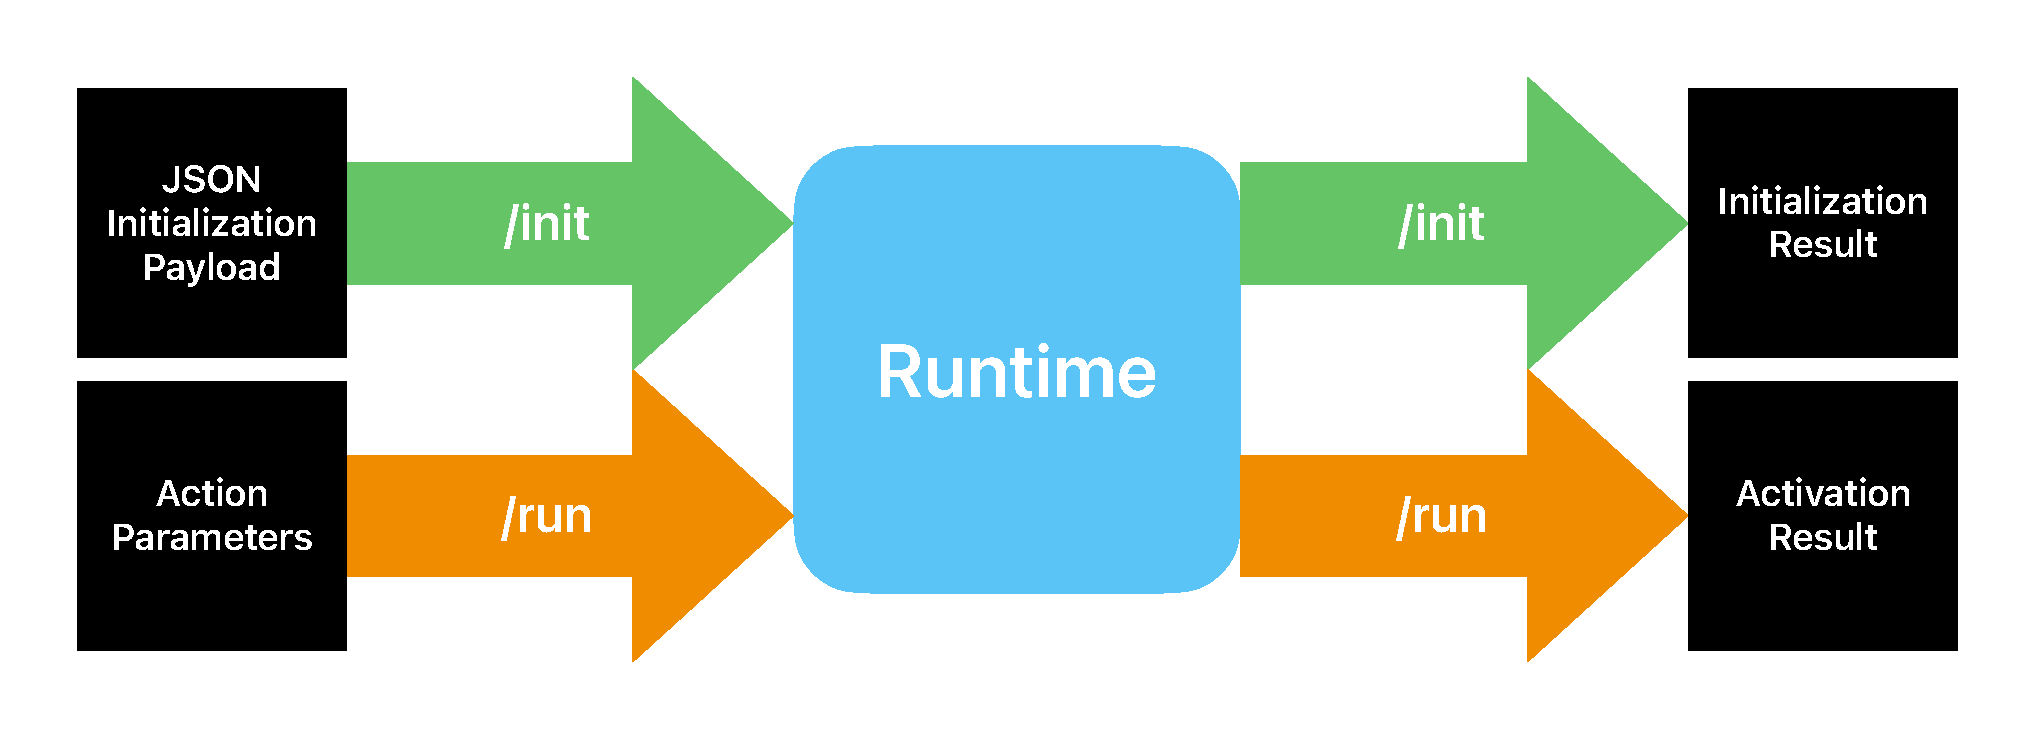
\includegraphics[width=\textwidth]{media/action_interface.pdf}
    \caption{Abstract representation of the Action Interface in OpenWhisk.}
    \label{fig:actioninterface}
\end{figure}

The /init endpoint is tasked with container initialization and accepts a POST request consisting of a JSON object that includes the action name, function to be executed, the source code, and several environment variables. This initialization happens exactly once and must be completed within a predefined time limit set by the platform \cite{action-interface}.

Once initialization is completed successfully, the runtime transitions to a state where it can activate the function. The /run endpoint is responsible for this task. It receives an HTTP POST request with a new activation context and the function's input parameters. The route needs to accept a JSON object and respond with one, adhering to the OpenWhisk platform's prescribed schema. Every action in OpenWhisk has a set time limit, within which the activation must complete. If the function executes successfully, the route responds with 200 OK, and the response body is recorded as the result of the activation \cite{openwhisk2023}.

The runtime should flush all the logs generated during initialization and execution, adding a unique frame marker at the end of each activation log stream. This marker is necessary to avoid delayed or truncated activation logs \cite{openwhisk2023}.

\subsection{ActionLoop Proxy in OpenWhisk}

The ActionLoop proxy is a tool designed to simplify the process of creating new OpenWhisk runtimes. While one can develop a new runtime by following the Action Interface, the ActionLoop proxy offers a quicker and more efficient way to achieve this by implementing most of the specification out-of-the-box \cite{action-proxy}.

The ActionLoop proxy is a runtime engine, developed in Go, initially designed to support the OpenWhisk Go language runtime. However, its generic design allows it to be adapted for other language runtimes such as Swift, PHP, Python, Rust, Java, Ruby, and Crystal. It was engineered keeping both compiled and scripting languages in mind.

Using the ActionLoop proxy, one can develop a new runtime in a fraction of the time it would take to create one from scratch. This is due to the fact that the ActionLoop proxy requires the developer to write only a command line protocol instead of a full-fledged web server, reducing complexity. Additionally, the ActionLoop proxy is known to significantly enhance the performance of existing runtimes, providing speed improvements ranging from 2x to 20x \cite{action-proxy}.

Since Swift, like all other language runtimes except Javascript, leverage it, understanding the ActioxnLoop proxy is crucial to be able to update the OpenWhisk runtime to support the latest version of Swift, enhancing the potential for Swift to be used as a Serverless language.

\subsection{Compiling a Swift action with the ActionLoop Proxy}
Runtimes are docker images. One of the features of the ActionLoop proxy is compiling an action into a binary file that can then be used by the runtime to run the action. This could be useful in debugging, as well as accelerating development.
Having the ability to compile locally is crucial in the development process. Developers can immediately catch any compile-time errors, which in the context of Swift and most statically typed languages, is especially useful since many errors are caught there. This effect is more pronounced in the case of Swift, as we will see in later chapters where we explain some of Swift's safety features.
Suppose the Swift runtime is built into the docker image tagged as swift-one. With the following command we can build the binary for the action that runs the fuction mainName:
\begin{minted}{bash}
docker run swift-one -compile mainName
\end{minted}
The standard input of this command is the source file of our function. There are two cases on where that function could reside:
\begin{description}
	\item [Single File] the function is contained in a single Swift file
	\item [Package] the function is part of a Swift package
\end{description}
In the case of the Swift package, it should be zipped and be given as standard input to the command. The Swift runtime expects to be able to unzip it, and in the resulting directory run \mintinline{bash}{swift build -c release}. This is extracted into a src directory inside the docker container. In the parent folder there exists a sample swift package skeleton. In the case that the contents of the zip file are nested inside another folder, when the runtime tries to run the swift build command, unexpected behavior will occur. That is because the swift compiler when it can't find the Package.swift file in the current directory, it searches up the hierarchy to find it, resulting in it trying to build the blank swift package (which will most likely not contained the desired function). In our experience, this has caused countless hours of debugging and trying to figure out what the problem is, because of unhelpful feedback such as "function X not found". Fully understanding the inner workings of the ActionLoop proxy and the Swift runtime was required. One could argue the simplicity the ActionLoop proxy aims to provide is lost in this.
The following command produces the binary executable fun for the function fun() which is contained in the Swift package which is zipped inside myPackage.zip:
\mint{bash}{docker run swift-one -compile fun <myPackage.zip >fun.zip}
fun.zip contains a folder which contains the actual binary.

The behavior of the binary is as follows: It listens on standard output for the JSON payload OpenWhisk will send it (which contains the parameters of the function). It writes to standard output the result of the function. In case that the output is a Codable type, it returns the JSON encoded text.


\section{Process of Updating the Swift Runtime}
\label{sec:UpdatingProcess}

The current Swift runtime repository ~\cite{swift-runtime} contains a folder called core which contains the files necessary to build the image for each swift version.
\begin{figure}[h]
    \centering
    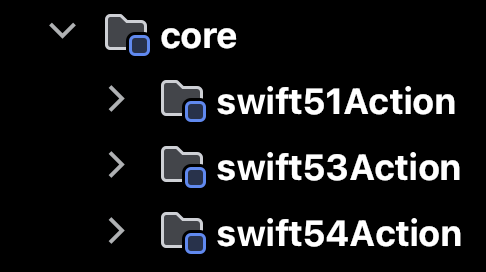
\includegraphics[width=\textwidth]{media/core_contents.png}
    \caption{Contents of the core folder of the Swift runtime}
    \label{fig:core_contents}
\end{figure}

Each folder contains the following files:
\begin{description}
	\item [Whisk.swift] A client for invoking actions, creating triggers, and most basic wsk functionalities in Swift. It is not directly needed in the runtime, but it is useful as a simple OpenWhisk SDK for swift.
	\item [build.gradle] Contains some gradle options. Mainly the name of the docker image (which will be built from this folder).
	\item [CHANGELOG.md] The changelog for that version.
	\item [main.swift] Contains just a sample function, used for testing and an initial swift build.
	\item [Dockerfile] The actual docker file for building the image. It is responsible for including the ActionLoop proxy.
	\item [Package.swift] Sample package file used for testing.
	\item [swiftbuild.py] This file is used as the /bin/compile tool, as specified in the ActionLoop proxy. It is responsible for creating the action binary.
	\item [swiftbuild.py.launcher.swift] This is used as the /bin/compile.launcher file, as specified in the ActionLoop proxy. This file contains all supported signatures for deploying functions.
	\item [swiftbuildandlink.sh]In the case of Swift, this just build the Swift executable
\end{description}
In order to actually update the runtime, a copy of any of the existing runtime folder will do, and requires minimal changes:
\begin{description}
	\item [Dockerfile] Simply replace the swift image tag to the latest one (FROM swift:5.4 -> FROM swift:5.8)
	\item [build.gradle] Change the image tag to a new one: ext.dockerImageName = 'action-swift-v5.4' -> ext.dockerImageName = 'action-swift-v5.8'
	\item [swiftbuild.py.launcher.swift] Replace the callback-based functions to async based ones
\end{description}

\begin{minted}{swift}
func _run_main<Out: Encodable>(mainFunction: ( @escaping (Out?, Error?) -> Void) -> Void, json: Data) {
	let resultHandler = { (out: Out?, error: Error?) in
		if let error = error {
			_whisk_print_error(message: "Action handler callback returned an error:", error: error)
			return
		}
		guard let out = out else {
			_whisk_print_error(message: "Action handler callback did not return response or error.", error: nil)
			return
		}
		do {
			let jsonData = try Whisk.jsonEncoder.encode(out)
			_whisk_print_result(jsonData: jsonData)
		} catch let error as EncodingError {
			_whisk_print_error(message: "JSONEncoder failed to encode Codable type to JSON string:", error: error)
			return
		} catch {
			_whisk_print_error(message: "Failed to execute action handler with error:", error: error)
			return
		}
	}
	let _ = mainFunction(resultHandler)
}
\end{minted}
\begin{minted}{swift}
func _run_main<Out: Encodable>(mainFunction: ()async -> (Out?, Error?), json: Data) async{
	let (out, error) = await mainFunction()
	if let error = error {
		_whisk_print_error(message: "Action handler callback returned an error:", error: error)
		return
	}
	guard let out = out else {
		_whisk_print_error(message: "Action handler callback did not return response or error.", error: nil)
		return
	}
	do {
		let jsonData = try Whisk.jsonEncoder.encode(out)
		_whisk_print_result(jsonData: jsonData)
	} catch let error as EncodingError {
		_whisk_print_error(message: "JSONEncoder failed to encode Codable type to JSON string:", error: error)
		return
	} catch {
		_whisk_print_error(message: "Failed to execute action handler with error:", error: error)
		return
	}
}
\end{minted}
Now, \begin{description}
	\item [swiftbuild.py] needs to be updated so that the code it injects calls the async function with the await keyword:
\end{description}
\mintinline{python}{code += f" _run_main(mainFunction: {main}, json: nil)\n"}
becomes:
\mintinline{python}{code += f" await _run_main(mainFunction: {main}, json: nil)\n"}
\section{Challenges Encountered}
\label{sec:Challenges}
While updating the runtime in hindsight did not require many changes, understanding how it all works together with the ActionLoop proxy to produce and run a binary required considerable effort. Issues arose frequently. Small mistakes rarely yield useful feedback. As mentioned before, a small change such as nesting the source file just one folder further, leads to confusing behavior.

For instance, consider how the current swift runtime processes an input. It reads a line from standard input, which is the JSON object OpenWhisk provides. That object, contains the parameters of the activation under the key 'value'. 
\begin{minted}{swift}
	let jsonData = try JSONSerialization.data(withJSONObject: parsed["value"] as Any, options: [])
\end{minted}

Deploying and activating function without parameters is supported by openwhisk and very much possible. What happens when a Swift action is activated with no parameters? The runtime tries to serialize the [value] key which in this case does not exist. The result is that JSONSerialization's data function throws an error, failing the activation. 


